\makeatletter
\ifx\du\undefined
  \newlength{\du}
\fi
\setlength{\du}{\unitlength}
\ifx\spacing\undefined
  \newlength{\spacing}
\fi
\setlength{\spacing}{60\unitlength}
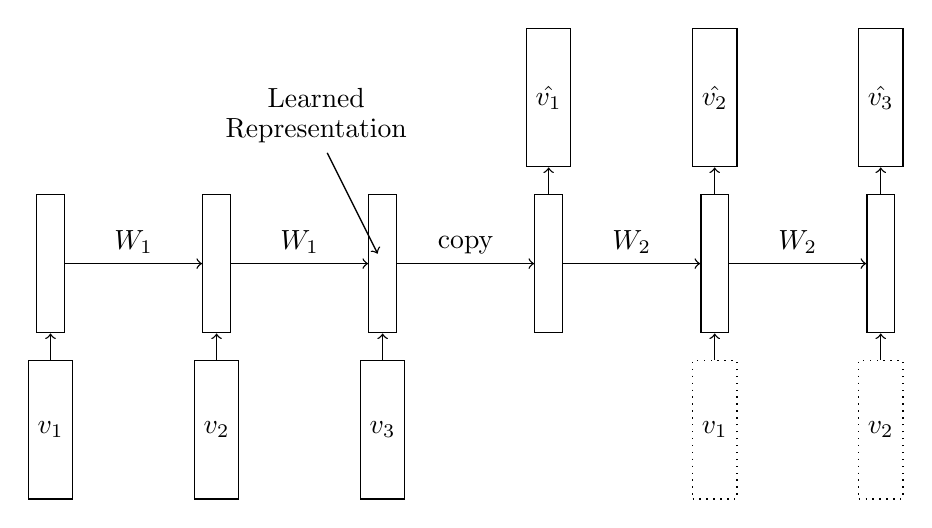
\begin{tikzpicture}
\pgfsetlinewidth{0.5\du}
\pgfsetmiterjoin
\pgfsetbuttcap

\node[rectangle, draw=black, minimum width=10\du, minimum height=50\du] (v1) at (0\spacing, 0) {$v_1$};
\node[rectangle, draw=black, minimum width=10\du, minimum height=50\du] (v2) at (\spacing, 0) {$v_2$};
\node[rectangle, draw=black, minimum width=10\du, minimum height=50\du] (v3) at (2\spacing, 0) {$v_3$};

\node[rectangle, dotted, draw=black, minimum width=10\du, minimum height=50\du] (v5) at (4\spacing, 0) {$v_1$};
\node[rectangle, dotted, draw=black, minimum width=10\du, minimum height=50\du] (v6) at (5\spacing, 0) {$v_2$};

\node[rectangle, draw=black, minimum width=10\du, minimum height=50\du] (h1) at (0\spacing, \spacing) {};
\node[rectangle, draw=black, minimum width=10\du, minimum height=50\du] (h2) at (\spacing, \spacing) {};
\node[rectangle, draw=black, minimum width=10\du, minimum height=50\du] (h3) at (2\spacing, \spacing) {};

\node[rectangle, draw=black, minimum width=10\du, minimum height=50\du] (h4) at (3\spacing, \spacing) {};
\node[rectangle, draw=black, minimum width=10\du, minimum height=50\du] (h5) at (4\spacing, \spacing) {};
\node[rectangle, draw=black, minimum width=10\du, minimum height=50\du] (h6) at (5\spacing, \spacing) {};

\node[rectangle, draw=black, minimum width=10\du, minimum height=50\du] (v4r) at (3\spacing, 2\spacing) {$\hat{v_1}$};
\node[rectangle, draw=black, minimum width=10\du, minimum height=50\du] (v5r) at (4\spacing, 2\spacing) {$\hat{v_2}$};
\node[rectangle, draw=black, minimum width=10\du, minimum height=50\du] (v6r) at (5\spacing, 2\spacing) {$\hat{v_3}$};

\node[anchor=center]  at (1.6\spacing, 2\spacing) {Learned};
\node[anchor=center] (p1) at (1.6\spacing, 1.8\spacing) {Representation};
\node[anchor=center] (p2) at (2\spacing, \spacing) {};
%\node[anchor=center] (w) at (0\spacing, 0.5\spacing) {$\WW_1$};

%\draw[ultra thick, ->] (2aa) -- node[left] {Conv Net} (3a);
\draw[->] (v1) -- (h1);
\draw[->] (v2) -- (h2);
\draw[->] (v3) -- (h3);
\draw[->] (v5) -- (h5);
\draw[->] (v6) -- (h6);

\draw[->] (h1) -- node[above] {$W_1$} (h2);
\draw[->] (h2) -- node[above] {$W_1$} (h3);
\draw[->] (h3) -- node[above] {copy} (h4);
\draw[->] (h4) -- node[above] {$W_2$} (h5);
\draw[->] (h5) -- node[above] {$W_2$} (h6);

\draw[->] (h4) -- (v4r);
\draw[->] (h5) -- (v5r);
\draw[->] (h6) -- (v6r);

\draw[->] (p1) -- (p2);
\end{tikzpicture}
